\documentclass{article}
\usepackage[italian]{babel}
\usepackage[utf8]{inputenc}
\usepackage{fancyhdr}
\usepackage{tikz}
\usepackage{amsmath}
\usepackage{amssymb}
\usepackage{amsthm}
\usepackage{amsfonts}
\usepackage{color}
\usepackage{circuitikz}
\usepackage[margin=2cm]{geometry}
\usepackage[scientific-notation=true]{siunitx}
\usepackage{titlesec}
\usepackage{graphics}

\titleformat{\paragraph}
  {\normalfont\normalsize\bfseries}{\theparagraph}{1em}{}
\titlespacing*{\paragraph}
  {0pt}{3.25ex plus 1ex minus .2ex}{1.5ex plus .2ex}

\title{Misura della caratteristica di un transistor BJT P-N-P in configurazione a emettitore comune}
\date{Quarto turno}
\author{Bertasi Leonardo, Perniola Davide }
\begin{document}
\maketitle
\section{Introduzione} 
Il transistor BJT è un dispositivo bipolare a tre terminali, costituito quindi da tre regioni di semiconduttore con drogaggio alternato
p-n-p o n-p-n. Le tre regioni sono chiamate emettitore, base e collettore. In questa prova abbiamo utilizzato transistor BJT 2N3906(BU) Silicio P-N-P in configuarzione a emettitore comune
e misurato, utilizzando due diverse correnti di base $I_B$, la caratteristica di uscita, ovvero la corrente di collettore $I_C$ in funzione della tensione tra collettore ed emettitore $V_{CE}$.
Inoltre durante la prova sono stati utilizzati due potenziometri da $100k\Omega$ e $1k\Omega$, un alimentatore di bassa tensione un multimetro digitale e un oscilloscopio.
Il circuito realizzato è riporato in Figura 1.



\begin{figure}[]
  \centering
  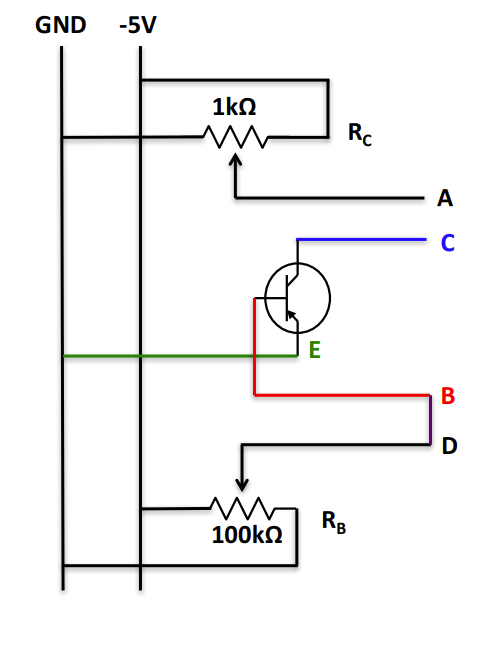
\includegraphics[scale=0.55]{Transis.png}
  \qquad
  \caption{\textit{Rappresentazione schematica del circuito realizzato. }}
\end{figure}



\section{Risultati}
Lo scopo di questa prova è stato misurare le caratterisrticge e 
Lo scopo di questa prova è stato misurare le caratterisrticge e 
Lo scopo di questa prova è stato misurare le caratterisrticge e 
Lo scopo di questa prova è stato misurare le caratterisrticge e 


\begin{table}[]
  \centering
 \mbox{%
\begin{tabular}{|c|c|c|}

\hline
$F.S(mV/div)$ & $V(mV)$ & $I(mA)$\\
\hline

$1000$ & $-4000\pm{156}$ & $-37.5\pm{0.6}$ \\
$1000$ & $-3800\pm{152}$ & $-36.6\pm{0.6}$ \\
$1000$ & $-3600\pm{147}$ & $-36.4\pm{0.6}$ \\
$500$ & $-3400\pm{114}$ & $-35.8\pm{0.5}$ \\
$500$ & $-3200\pm{108}$ & $-35.6\pm{0.5}$ \\
$500$ & $-3000\pm{103}$ & $-35.5\pm{0.5}$ \\
$500$ & $-2800\pm{98}$ & $-35.1\pm{0.5}$ \\
$500$ & $-2600\pm{93}$ & $-34.7\pm{0.5}$ \\
$500$ & $-2400\pm{88}$ & $-34.5\pm{0.5}$ \\
$500$ & $-2200\pm{83}$ & $-34.1\pm{0.5}$ \\
$500$ & $-2000\pm{78}$ & $-33.8\pm{0.5}$ \\
$500$ & $-1800\pm{74}$ & $-33.3\pm{0.5}$ \\
$500$ & $-1600\pm{69}$ & $-32.8\pm{0.5}$ \\
$500$ & $-1400\pm{65}$ & $-32.6\pm{0.5}$ \\
$500$ & $-1200\pm{62}$ & $-32.0\pm{0.5}$ \\
$500$ & $-1000\pm{58}$ & $-31.5\pm{0.5}$ \\
$500$ & $-900\pm{57}$ & $-31.1\pm{0.5}$ \\
$500$ & $-800\pm{55}$ & $-30.7\pm{0.5}$ \\
$500$ & $-700\pm{54}$ & $-30.2\pm{0.5}$ \\
$500$ & $-600\pm{53}$ & $-29.4\pm{0.5}$ \\
$200$ & $-500\pm{25}$ & $-28.6\pm{0.4}$ \\
$100$ & $-450\pm{17}$ & $-27.5\pm{0.4}$ \\
$100$ & $-400\pm{16}$ & $-26.7\pm{0.4}$ \\
$100$ & $-350\pm{15}$ & $-25.8\pm{0.4}$ \\
$100$ & $-300\pm{13}$ & $-24.6\pm{0.4}$ \\
$100$ & $-250\pm{13}$ & $-22.9\pm{0.4}$ \\
$100$ & $-200\pm{12}$ & $-20.7\pm{0.3}$ \\
$100$ & $-150\pm{11}$ & $-15.0\pm{0.2}$ \\
$100$ & $-100\pm{10}$ & $-9.2\pm{0.1}$ \\
$50$ & $-80\pm{6}$ & $-4.4\pm{0.1}$ \\
$50$ & $-60\pm{5}$ & $-2.3\pm{0.1}$ \\
$50$ & $-50\pm{5}$ & $-1.43\pm{0.1}$ \\

\hline
\end{tabular}
 }
 \caption{\textit{Risultati delle misure effettuate con il diodo al silicio. Sono riportate i valori di corrente e delle differenze di potenziale corrispettive, oltre che il fondo scale scelto per ogni misura}}
\end{table}

Tebelleee


\begin{table}[]
  \centering
 \mbox{%
\begin{tabular}{|c|c|c|}

\hline
$F.S(mV/div)$ & $V(mV)$ & $I(mA)$\\
\hline

$1000$ & $-4000\pm{156}$ & $-19.3\pm{0.3}$ \\
$1000$ & $-3800\pm{152}$ & $-19.3\pm{0.3}$ \\
$1000$ & $-3600\pm{147}$ & $-19.2\pm{0.3}$ \\
$500$ & $-3400\pm{114}$ & $-19.1\pm{0.3}$ \\
$500$ & $-3200\pm{108}$ & $-19.1\pm{0.3}$ \\
$500$ & $-3000\pm{103}$ & $-19.0\pm{0.3}$ \\
$500$ & $-2800\pm{98}$ & $-18.9\pm{0.3}$ \\
$500$ & $-2600\pm{93}$ & $-18.6\pm{0.3}$ \\
$500$ & $-2400\pm{88}$ & $-18.5\pm{0.3}$ \\
$500$ & $-2200\pm{83}$ & $-18.4\pm{0.3}$ \\
$500$ & $-2000\pm{78}$ & $-18.2\pm{0.3}$ \\
$500$ & $-1800\pm{74}$ & $-17.9\pm{0.3}$ \\
$500$ & $-1600\pm{69}$ & $-17.7\pm{0.3}$ \\
$500$ & $-1400\pm{65}$ & $-17.5\pm{0.3}$ \\
$500$ & $-1200\pm{62}$ & $-17.3\pm{0.3}$ \\
$500$ & $-1000\pm{58}$ & $-17.2\pm{0.3}$ \\
$500$ & $-900\pm{57}$ & $-17.0\pm{0.3}$ \\
$500$ & $-800\pm{55}$ & $-16.9\pm{0.3}$ \\
$500$ & $-700\pm{54}$ & $-16.8\pm{0.3}$ \\
$500$ & $-600\pm{53}$ & $-16.7\pm{0.3}$ \\
$200$ & $-500\pm{25}$ & $-16.5\pm{0.3}$ \\
$100$ & $-450\pm{17}$ & $-16.4\pm{0.3}$ \\
$100$ & $-400\pm{16}$ & $-16.2\pm{0.3}$ \\
$100$ & $-350\pm{15}$ & $-16.0\pm{0.3}$ \\
$100$ & $-300\pm{13}$ & $-15.5\pm{0.2}$ \\
$100$ & $-250\pm{13}$ & $-14.7\pm{0.2}$ \\
$100$ & $-200\pm{12}$ & $-13.9\pm{0.2}$ \\
$100$ & $-150\pm{11}$ & $-11.2\pm{0.2}$ \\
$100$ & $-100\pm{10}$ & $-6.1\pm{0.1}$ \\
$50$ & $-80\pm{6}$ & $-2.8\pm{0.1}$ \\
$50$ & $-60\pm{5}$ & $-1.3\pm{0.1}$ \\
$50$ & $-50\pm{5}$ & $-0.8\pm{0.1}$ \\

\hline
\end{tabular}
 }
 \caption{\textit{Risultati delle misure effettuate con il diodo al silicio. Sono riportate i valori di corrente e delle differenze di potenziale corrispettive, oltre che il fondo scale scelto per ogni misura}}
\end{table}


\section{Conclusioni}


Lo scopo di questa prova è stato misurare le caratterisrticge e 
Lo scopo di questa prova è stato misurare le caratterisrticge e 
Lo scopo di questa prova è stato misurare le caratterisrticge e 
Lo scopo di questa prova è stato misurare le caratterisrticge e 









\end{document}
